\documentclass[a4paper]{article}

%% Language and font encodings
\usepackage[english]{babel}
\usepackage[utf8x]{inputenc}
\usepackage[T1]{fontenc}

%% Sets page size and margins
\usepackage[a4paper,top=3cm,bottom=2cm,left=3cm,right=3cm,marginparwidth=1.75cm]{geometry}

%% Useful packages
\usepackage{amsmath}
\usepackage{graphicx}
\usepackage[colorinlistoftodos]{todonotes}
\usepackage[colorlinks=true, allcolors=blue]{hyperref}

\title{GUI for Image Processing}
\author{Carina Vallefuoco}

\begin{document}
\maketitle

\begin{abstract}
This manual will explain step by step how to process an image with Matlab's GUI.
\end{abstract}

\section{Introduction}

This project uses Matlab's built in GUIs (also known as graphical user interfaces or UIs) which provides an easy point-and-click technique to manage software applications. With GUIs anyone can run applications which having much knowledge in type command or coding languages. 

\section{Creating a GUI}
\subsection{How to create a GUIDE}

To create a GUI we use a GUIDE (GUI development environment) which provides tools to graphically design a custom app. GUIDE automatically generates the MATLAB code for a GUI which can be modified to the desired behavior of your app.
To create your GUIDE go to the command window and type in GUIDE. In the GUIDE Quick Start dialog box, select the Blank GUI (Default) template, and then click OK. To display the names of the components in the component palette: Select File > Preferences. Then, check the box for the component palette, click apply then ok (See figure 1).

\section{Component Palette}
\subsection{How to create an Axes}

To create a space for an image click on the Axes button located in the component palette. click and drag to create a square box (See figure 1). The size and placement can be modified during any point of the design.

\begin{figure}
\centering
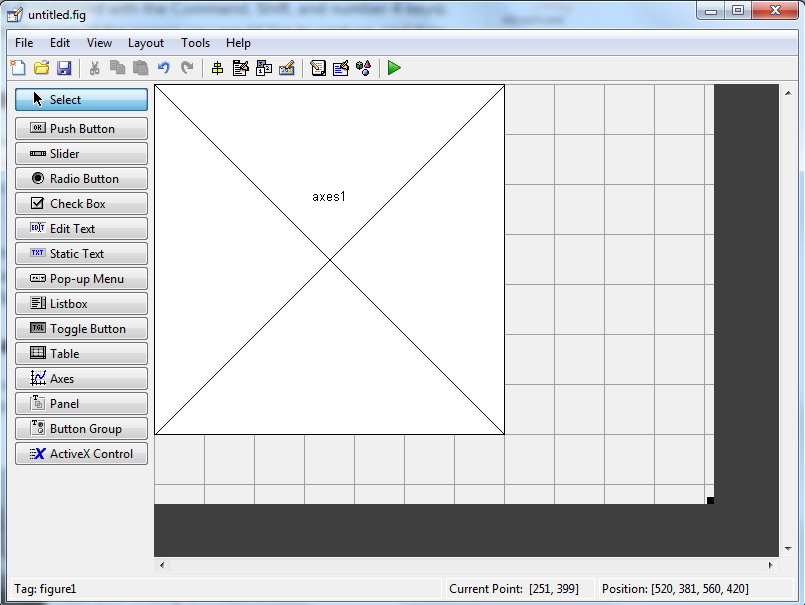
\includegraphics[width=0.3\textwidth]{Capture.PNG}
\caption{\label{fig:GUI}This is a GUIDE with an axis added.}
\end{figure}

\subsection{How to create Push Buttons}

Add push button from the component palette and drag them to the desired location. to modify the text in them left click on the selected push button and then click property inspector. From there you will see 'String' in the left column and 'Push Button' in the right column. By selecting the 'Push Button' you can then edit the text (See figure 2).The size and placement of a push button can be modified during any point of the design.

\begin{figure}
\centering
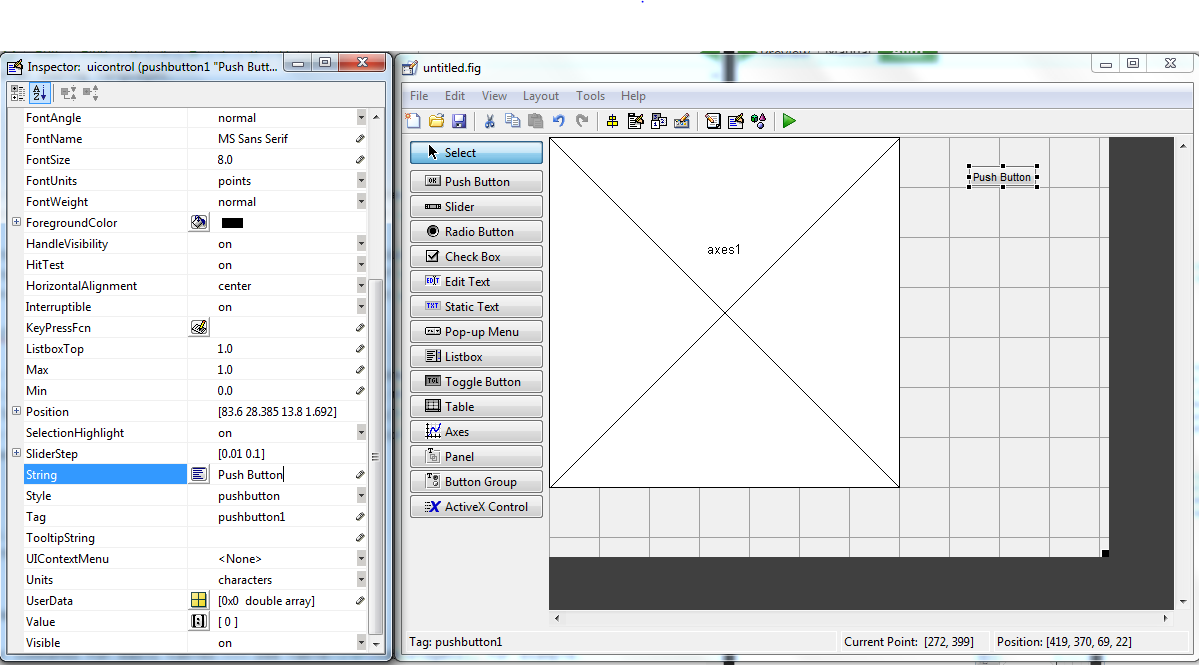
\includegraphics[width=0.3\textwidth]{Capture1.PNG}
\caption{\label{fig:Push Button}To edit the name of a push button.}
\end{figure}

\subsection{How to add a Slide bar}
Select the slider button from the component palette and drag and drop it to the desired location (See figure 3).The size and placement can be modified during any point of the design.

\begin{figure}
\centering
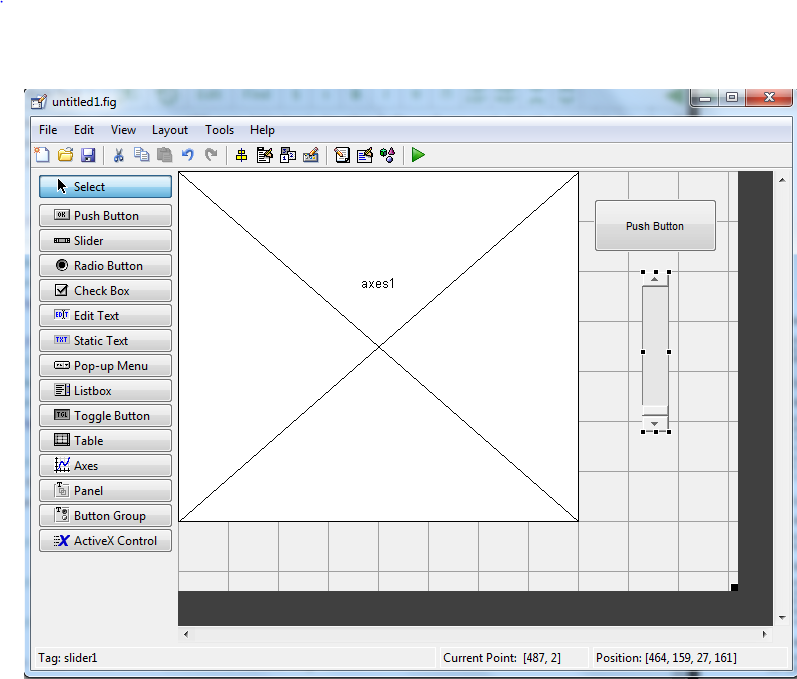
\includegraphics[width=0.3\textwidth]{Capture2.PNG}
\caption{\label{fig:Slide Bar}Slide Bar.}
\end{figure}

\subsection{How to add Static Text}
Add static text from the component palette and drag it to the desired location. to modify the text in them left click on the selected static text and then click property inspector. From there you will see 'String' in the left column and 'Static Text' in the right column. By selecting the 'Static Text' you can then edit the text (See figure 4).The size and placement can be modified during any point of the design.

\begin{figure}
\centering
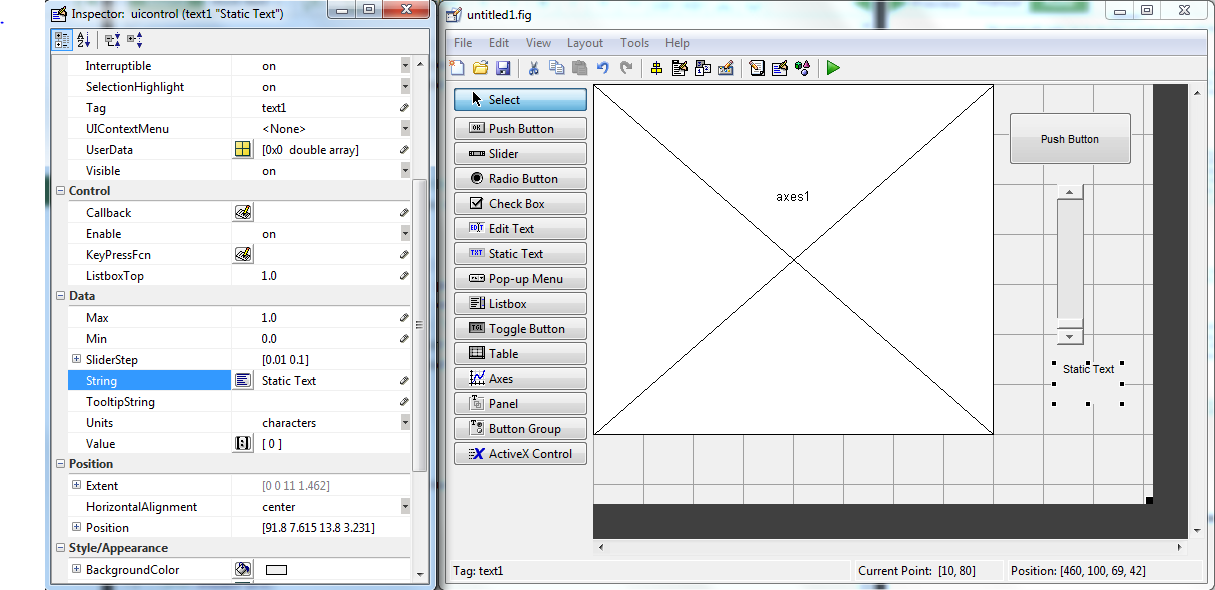
\includegraphics[width=0.3\textwidth]{Capture3.PNG}
\caption{\label{fig:Static Text}Static Text.}
\end{figure}

\section{Matlab Coding}
To control each push button and slide bar we must code each one in the .m file that is automatically generated when we create a GUI through the GUIDE.

\subsection{How to Load an Image}
To load an image we use imgetfile() to get the path of the file > imread() to read the file > im2double() to convert to double precision. Then we save an extra copy of the image for back-up. Check out finalGUI.m for Matlab code.

\subsection{How to Reset an Image}
The back-up image that was saved during the loading function will be used to rest the image back to the original. Check out finalGUI.m for Matlab code.

\subsection{How to Apply Grayscale to an Image}
Simply by subtracting the image from 1 (1-image), we can obtain a grayscaled image. Check out finalGUI.m for Matlab code.

\subsection{How to Apply a Wave to an Image}
Going through each row and column of the image we can use an amplitude of 50 and a frequency of 1/30 to apply to each row by multiplying the frequency to the column element and taking the cosine value of that and multiplying it by the amplitude and adding the row element. We will use floor() to round towards minus infinity and set the bounds so the wave doesn't go outside the borders of the image. Check out finalGUI.m for Matlab code.

\subsection{How to Modify Brightness to an Image}
Use the slider bar to adjust the brightness. We use get() to get the value the user chooses and multiply that by .5 then subtract .5. Then we add that value to the image.  Check out finalGUI.m for Matlab code.


\subsection{How to save an Image}
To save the image you can use copyobj() to copy the image and saveas() to save the image to your desktop. Check out finalGUI.m for Matlab code.

\section{Warhol Pop Art}
Andy Warhol was an American artist who lead the visual art movement with pop art. Pop art is an art movement in the mid-1950s in Britain and the late 1950s in the United States. Warhol used pop art to illustrate large themes of public life and society. See figure 5,6, and 7 for some of his most popular and well-known work.

\begin{figure}
\centering
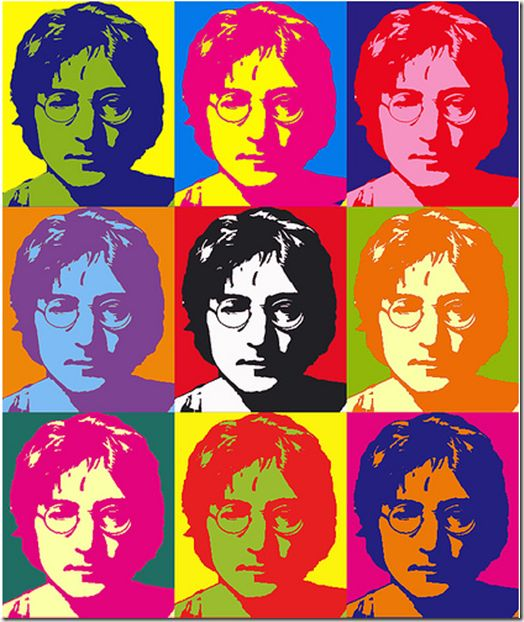
\includegraphics[width=0.3\textwidth]{ex1.jpg}
\caption{\label{fig:Warhol example 1}}
\end{figure}

\begin{figure}
\centering
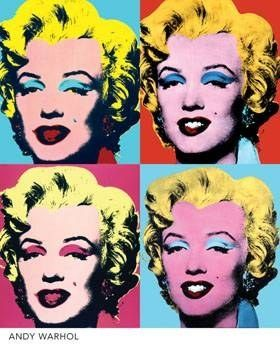
\includegraphics[width=0.3\textwidth]{ex2.jpg}
\caption{\label{fig:Warhol example 2}}
\end{figure}

\begin{figure}
\centering
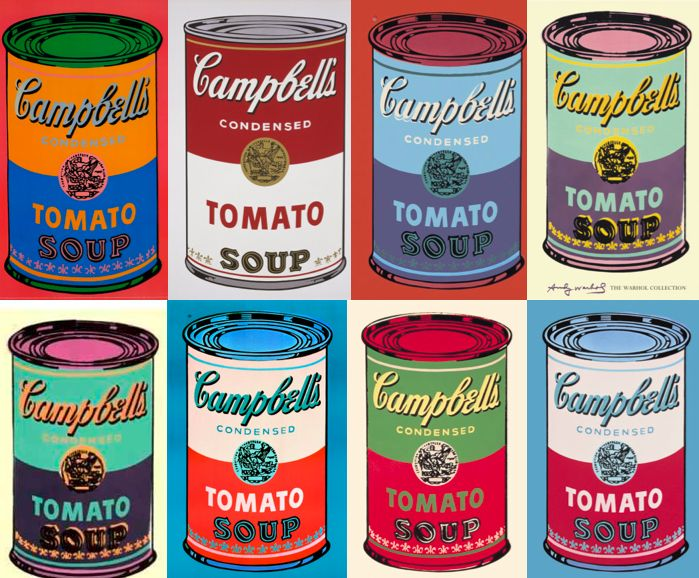
\includegraphics[width=0.3\textwidth]{ex3.jpg}
\caption{\label{fig:Warhol example 3}}
\end{figure}

\subsection{How to Create a 2x2 Pop Art}
To create pop art similar to Warhol's artwork we can switch the red, green, and blue layers of an image. Then creating a matrix of the new image and the old image we get a collage of Matlab generated pop art (See figure 8 for 2x2 pop art i made in Matlab)! Check out finalGUI.m for Matlab code.

\begin{figure}
\centering
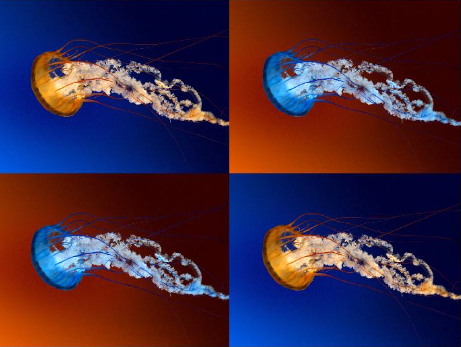
\includegraphics[width=0.3\textwidth]{vallex1.PNG}
\caption{\label{fig:Vallefuoco example 1}}
\end{figure}

\subsection{How to Create a 2x3 Pop Art}
To create a 2x3 pop art you use the same process as a 2x2 but instead of only making one new image with the color layers switched you create two images with different colors switched.(See figure 9 for 2x3 pop art i made in Matlab)! Check out finalGUI.m for Matlab code.

\begin{figure}
\centering
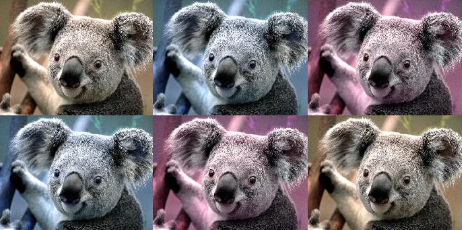
\includegraphics[width=0.3\textwidth]{vallex2.PNG}
\caption{\label{fig:Vallefuoco example 2}}
\end{figure}

\section{Future Goals}
In the future I would like to be able to allow more variations with the pop art options. I could create push button for certain flips of color layers. So instead of the preset function that changes just two colors it allows the user to select what colors they would like to switch. I would also like to add more options for dimensions i.e. 3x3, 5x5, 10x10, etc.






\end{document}